\documentclass[12pt,letterpaper]{article}
\usepackage[margin=1in]{geometry}
\usepackage{amsfonts}
\usepackage{amssymb}
\usepackage{amsthm}
\usepackage{amsmath}
\usepackage{enumerate}

%Here are some user-defined notations
\newcommand{\RR}{\mathbf R}  %bold R
\newcommand{\CC}{\mathbf C}  %bold C
\newcommand{\ZZ}{\mathbf Z}   %bold Z
\newcommand{\QQ}{\mathbf Q}   %bold Q
\newcommand{\rr}{\mathbb R}     %blackboard bold R
\newcommand{\cc}{\mathbb C}    %blackboard bold R
\newcommand{\zz}{\mathbb Z}    %blackboard bold R
\newcommand{\qq}{\mathbb Q}   %blackboard bold Q
\newcommand{\calM}{\mathcal M}  %calligraphic M
\newcommand{\sm}{\setminus} 
\newcommand{\bfa}{\mathbf a}
\newcommand{\bfb}{\mathbf b}
\newcommand{\bfc}{\mathbf c}


\usepackage{tikz}
\usetikzlibrary{positioning}
\usepackage{graphicx}


%Here are some user-defined operators
\newcommand{\re}{\operatorname {Re}}
\newcommand{\im}{\operatorname {Im}}


%These commands deal with theorem-like environments (i.e., italic)
\theoremstyle{plain}
\newtheorem{theorem}{Theorem}[section]
\newtheorem{corollary}[theorem]{Corollary}
\newtheorem{lemma}[theorem]{Lemma}
\newtheorem{conjecture}[theorem]{Conjecture}

%These deal with definition-like environments (i.e., non-italic)
\theoremstyle{definition}
\newtheorem{definition}[theorem]{Definition}
\newtheorem{example}[theorem]{Example}
\newtheorem{remark}[theorem]{Remark}

%your name and date in the header.
\usepackage[us]{datetime} 
\usepackage{fancyhdr}
\pagestyle{fancy}
\lhead{}
\chead{MATH 2710\\ Homework 4}
\rhead{ Your name \\ Oct. 26 2016}
\lfoot{}
\cfoot{}
\rfoot{\thepage}
\renewcommand{\headrulewidth}{0 pt}
\renewcommand{\footrulewidth}{0 pt}
\begin{document}
\ \\
\begin{enumerate}[1.]
\item A sequence of integers $x_1, x_2, x_3,\ldots $ is defined recursively by $x_1=3$, $x_2=7$ and
\[x_k=5x_{k-1}-6x_{k-2}\ \ \text{ for all }k\geq 3\]
Prove by induction that $x_n=2^n+3^{n-1}$ for all positive integers $n$. 
\ \\
\item Prove by induction that a set of $n$ elements contains $2^n$ subsets (including the set itself and $\emptyset$).
\ \\
\item Prove by induction that if $n$ points lie in a plane and no three are colinear, prove that there are $\frac{1}{2}n(n-1)$ lines joining these points. \\
\ \\
{\bf Example: }
\begin{center}
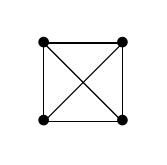
\begin{tikzpicture}
\node at (0,0){$\bullet$};
\node at (1,0){$\bullet$};
\node at (0,1){$\bullet$};
\node at (1,1){$\bullet$};
\draw (1,1)--(0,0) ;
\draw (1,0)--(0,0) ;
\draw (1,1)--(1,0) ;
\draw (0,1)--(0,0) ;
\draw (0,1)--(1,1) ;
\draw (0,1)--(1,0) ;
\end{tikzpicture}
\end{center}

\item Suppose that n chords are drawn in a circle, dividing the circle into different regions.
Prove that every region can be colored one of two colors such that adjacent regions are
different colors. \\
\ \\
{\bf Example: }
\begin{center}
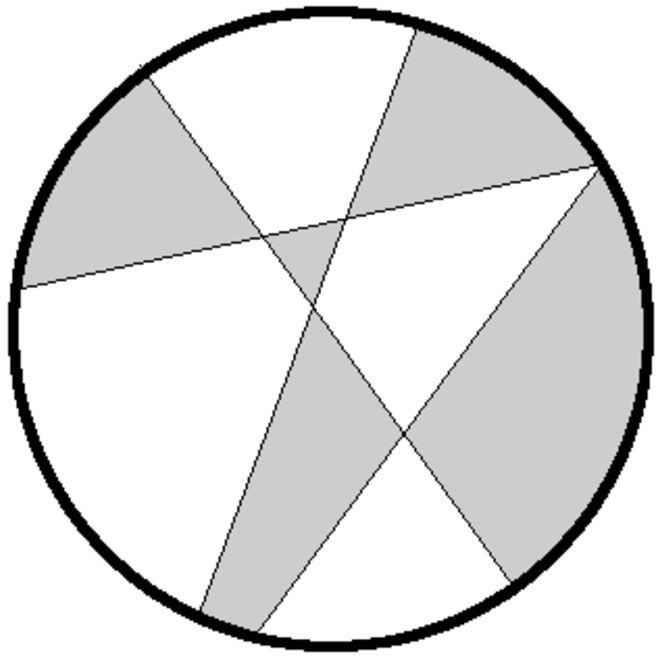
\includegraphics[scale=0.25]{circle}
\end{center}


\item  Prove that multiplication is a well defined operation on $\mathbb{Q}$.
\ \\
\item Prove that $\sqrt{3}$ is irrational. 

\end{enumerate}

\end{document}








